\begin{figure}[tb]
\centering
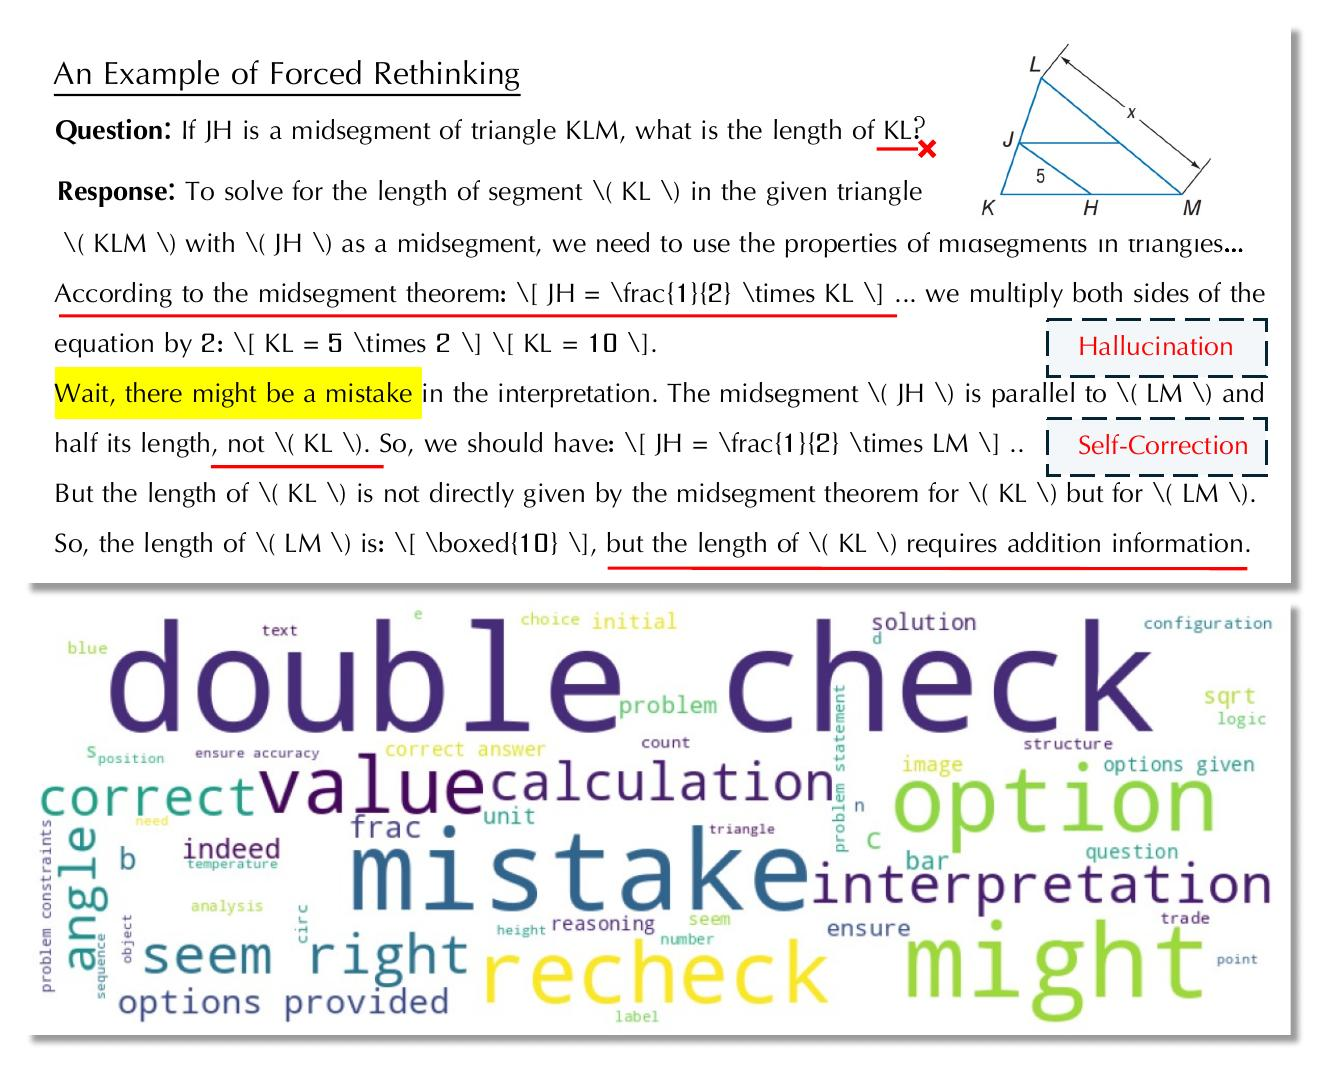
\includegraphics[width=\linewidth,height=0.3\textheight,keepaspectratio]{figures/rethinking.jpg}
\caption{\small \textbf{Forced Rethinking in practice.} \emph{Top:} a response from training with Forced Rethinking. The initial reasoning misapplies the midsegment theorem (JH $=\tfrac12$KL, a hallucinated relation). After the appended trigger ``Wait, there might be a mistake'', the model notices that JH is parallel to and half of LM, not KL, and revises its conclusion (self-correction). \emph{Bottom:} word cloud of the rethinking segments, dominated by verification and correction phrases (``double check'', ``mistake'', ``recheck'', ``might'', ``seem right'').}
\label{fig:rethinking}
\end{figure}
